\documentclass[11pt]{beamer}
\usetheme{Montpellier}
\usecolortheme{orchid}
\usepackage[utf8]{inputenc}
\usepackage[german]{babel}
\usepackage[T1]{fontenc}
\usepackage{amsmath}
\usepackage{amsfonts}
\usepackage{amssymb}
\usepackage{graphicx}
\usepackage{url}
\usepackage[export]{adjustbox}

\usepackage{tikz}
\usetikzlibrary{positioning, arrows}
\tikzset{
block/.style={
  draw, 
  rectangle, 
  minimum height=1.5cm, 
  minimum width=3cm, align=center
  }, 
line/.style={->,>=latex'}
}
\def\checkmark{\tikz\fill[fill=green!50!black,scale=0.4](0,.35) -- (.25,0) -- (1,.75) -- (.25,.15) -- cycle;} 

\author{Patrick M\"unnich}
\title{Identifizierung des Sigmatismus Lateralis in Audioaufnahmen}
%\setbeamercovered{transparent}
\setbeamertemplate{navigation symbols}{} 
\institute{Hochschule D\"usseldorf} 
%\date{} 
\subject{Signalverarbeitung} 
\begin{document}

%\begin{frame}
%\titlepage
%\end{frame}

\section{Inhaltsverzeichnis}

\begin{frame}
\tableofcontents
\end{frame}

\section{Sigmatismus Lateralis}

\begin{frame}
\frametitle{Sigmatismus Lateralis}
\begin{figure}
%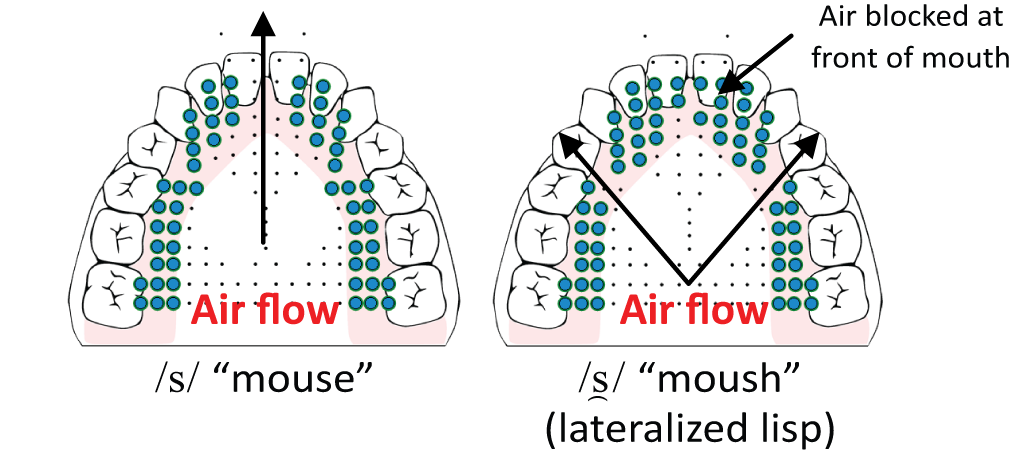
\includegraphics[scale=0.4]{lateral_lisp.png}
\begin{tikzpicture}[baseline=(current bounding box.north)]
\begin{scope}
    \clip (-2,0) rectangle (2,2);
    \draw (0,0) circle(2);
    \draw (-2,0) -- (2,0);
\end{scope}
\draw[line] (0,0) -> (0,3);
\begin{scope}
    \clip (3,0) rectangle (7,2);
    \draw (5,0) circle(2);
    \draw (3,0) -- (7,0);
\end{scope}
\draw[line] (5,0) -> (7,3);
\draw[line] (5,0) -> (3,3);
\node[below= 1mm of {(0,0)}] {Normales S};
\node[below= 1mm of {(5,0)}] {Sigmatismus Lateralis};
\end{tikzpicture}
\caption{Luftausbreitung von normalem ''s'' (S) und Sigmatismus Lateralis (SL).}% (\url{https://www.pinterest.com/pin/7248049373293660/})}
\end{figure}
\end{frame}

\begin{frame}
\frametitle{Sigmatismus Lateralis Video}
\centering
\url{https://youtu.be/Y3mEaV1kCiU?t=21}
\end{frame}

\section{Vergleich von FFTs}

\subsection{Parameter}

\begin{frame}
\frametitle{Parameter}
\begin{itemize}
\item Einfache Aufnahme mit Clip-on Mikrofon neben Mund
\item 16-bit mono mit $f_\mathrm{sampling}=8000$\,Hz
\item Insgesamt drei Aufnahmen
\item Alle Aufnahmen nur stimmloses ''s'' Ger"ausch mit oder ohne Lispeln\
\item Neu: betrachten von kleineren Fenstern, z.B.\ 1\,s
\end{itemize}
\end{frame}

\subsection{Vergleich}

\begin{frame}
\frametitle{Vergleich von FFTs}
\begin{figure}
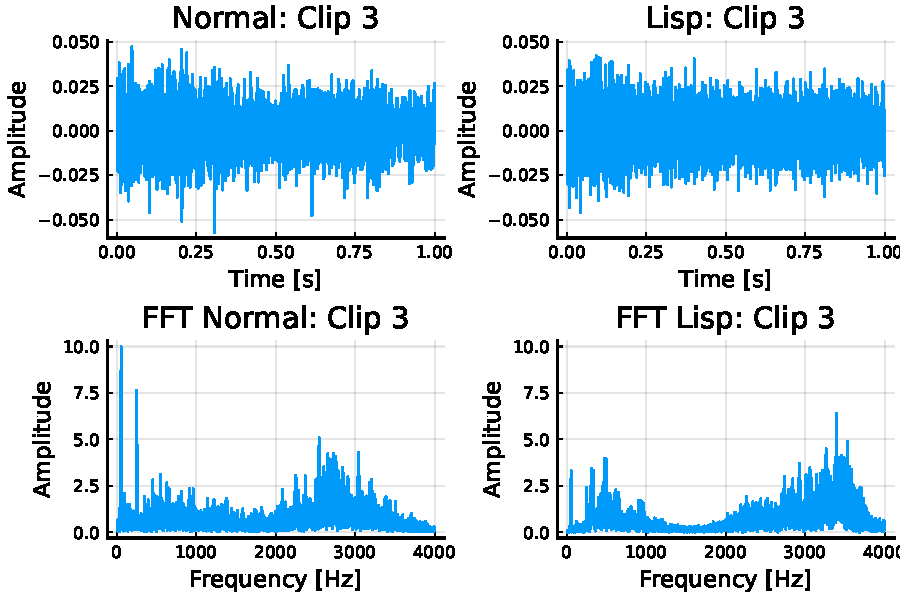
\includegraphics[scale=0.5]{../output/normal_vs_lisp_clip_3.pdf}
\caption{Beispielsweiser Vergleich der FFTs von S und SL.}
\end{figure}
\end{frame}

\subsection{Analyse}

\begin{frame}
\frametitle{Feststellungen bei Vergleich von FFTs}
\begin{itemize}
\item Erh"ohung im Bereich von ca 3000-3500\,Hz bei SL, 2500-3000\,Hz bei S 
\item Ansatz: man sollte durch Vergleich dieses Frequenzbands zwischen S und SL unterscheiden k"onnen
\end{itemize}
\end{frame}

\begin{frame}
\frametitle{Codediagramm}
\begin{figure}
\scalebox{0.5}{
\begin{tikzpicture}

\node[block]	(read)														{Audiodatei \\ einlesen};
\node[block]	(parameters)		[above right=0.2cm and 2cm of read]			{Parameter \\ feststellen};
\node[block]	(subtraction)	[below right=0.2cm and 2cm of read]			{Subtraktion des \\ Mittelwerts};
\node[block]	(normalizesub)	[right=of subtraction]						{Normalisierung};
\node[block]	(absfft)			[right=of normalizesub]						{Absolutwerte \\ FFT};
\node[block]	(slice)			[below right=1cm and 2cm of absfft]			{Begrenzung auf \\ Frequenzband};
\node[block]	(plot)			[above=4.5cm of slice]						{Plotten};
\node[block]	(normalizefft)	[left=of slice]								{Normalisierung};
\node[block]	(split)			[left=of normalizefft]						{Aufspaltung \\ Band und Rest};
\node[block]	(mean)			[left=of split]								{Mittelwerte \\ berechnen};
\node[block]	(thresh)			[left=of mean]							{Differenz $> 0$ \\ $\Rightarrow$ Lisp};

\draw[line] 	(read.north) 		|- 	(parameters.west);
\draw[line] 	(read.south) 		|- 	(subtraction.west);
\draw[line]	(subtraction.east) 	--	(normalizesub.west);
\draw[line] 	(normalizesub.east) 	--	(absfft.west);
\draw[line] 	(absfft.east) 		-|	(plot.south);
\draw[line] 	(absfft.east) 		-|	(slice.north);
\draw[line] 	(parameters.east)	--	(plot.west);
\draw[line] 	(slice.west)			--	(normalizefft.east);
\draw[line] 	(normalizefft.west) 	-- 	(split.east);
\draw[line] 	(split.west)			--	(mean.east);
\draw[line] 	(mean.west) 			-- 	(thresh.east);
\end{tikzpicture}
}
\caption{Funktionsweise des derzeitigen Codes zur Identifizierung des SL in Aufnahmen}
\end{figure}\label{examinesegment}
\end{frame}

\begin{frame}
\frametitle{Ergebnisse}
\begin{exampleblock}{Einfache Parameter}
Bei den derzeitigen einfachen Parametern kann der Code beide ''s'' Formen identifizieren.
\end{exampleblock}

\begin{block}{Implementierung in Julia}
\url{https://github.com/munnich/lateral-lisp}
\end{block}
\end{frame}

\subsection{Einf\"uhrung anderer Parameter}

\begin{frame}
\frametitle{Vergleich mit \textit{AT2020USB+} Mikrophon}
\begin{figure}
\includegraphics[scale=0.5]{../output/normal_vs_lisp_at_1.pdf}
\caption{Beispielsweiser Vergleich mit \textit{AT2020USB+}. Ergebnisse "ahneln den vorherigen.}
\end{figure}
\end{frame}

\begin{frame}
\frametitle{Fenstergr"o"se}
Der derzeitige Algorithmus scheint bei den Aufnahmen sowohl bei L"angen von 5\,s als auch 0.5\,s die Formen korrekt zu identifizieren.
\end{frame}

\section{Ganze Texte}

\begin{frame}
\frametitle{Ganze Texte}
\begin{enumerate}
\item Audiodatei in Segmente aufspalten
\item Algorithmus aus \ref{examinesegment} mit
\begin{align*}
F_\mathrm{S} &= [2500, 3000]\,\mathrm{Hz} & F_\mathrm{SL} &= [3000, 4000]\,\mathrm{Hz}
\end{align*}
\item Bestimmung Anzahl SL > Anzahl S
\end{enumerate}
\end{frame}

\begin{frame}
\frametitle{Ergebnisse}
\begin{itemize}
\item 60\% der Texte korrekt zugeordnet
\item tendenziell mehr inkorrekt identifizierte S als SL
\end{itemize}
\end{frame}

%\section{Plan}
%
%\begin{frame}
%	\frametitle{Plan}
%	\begin{enumerate}
%		\item Identifizierung SL durch Vergleich der Durchschnittsamplitude im Bereich 1200-3500\,Hz \checkmark
%		\item Einf"uhrung verschiedener Parameter, z.B.\ Mikrofon \checkmark, L"ange \checkmark, Lautst"arke etc.\ und Anpassung der bisherigen Methode
%		\item Identifizierung SL ohne Referenz-S \checkmark
%		\item[\textcolor{purple}{2.}] Identifizierung eines ''s'' in einem Wort, Fenster finden und entwickeltes Verfahren anwenden 
%	\end{enumerate}
%\end{frame}
%
%\section{Formanten}
%
%\begin{frame}
%\frametitle{Betrachtung der Formanten mit Praat}
%Screenshots w"aren hier leider zu gro"s
%\begin{block}{Ergebnisse}
%\begin{enumerate}
%\item Formant normal zwischen 700-800, Lispeln 500-700
%\item Formant normal zwischen 1500-2000, Lispeln 1800-2200
%\item[$\Rightarrow$] Schien konsistent "uber alle Aufnahmen
%\end{enumerate}
%\end{block}
%\end{frame}

\end{document}